% ==============================================================================
% #region Description and metadata of the report:
\title{Numerical and experimental study of the thermo-hydro-mechanical behavior of concrete under severe accident conditions using a poro-mechanical approach}

\author{Tan Kiet HONG}

\date{Grenoble, June 2026}

% ---- Custom fields ----
\makeatletter

\newcommand{\institution}[1]{\def\@institution{#1}}
\newcommand{\supervisors}[1]{\def\@supervisors{#1}}
\newcommand{\institutioninfo}[1]{\def\@institutioninfo{#1}}

\def\@institution{}
\def\@supervisors{}
\def\@institutioninfo{}

\makeatother

% ---- Fill data ----
\institution{UNIVERSITÉ GRENOBLE ALPES}

\supervisors{
Prof. Julien BAROTH, Université Grenoble Alpes\\[0.4cm]
Prof. Stefano DAL PONT, Université Grenoble Alpes
}

\institutioninfo{
This thesis is submitted in partial fulfillment of the requirements for the Master's degree in the International Program ``Geomechanics, Civil Engineering and Risks''.

\vspace{0.4cm}

The work was carried out during the Master 2 internship at 3SR Laboratory.
}

% This report presents the results of a Master 2 internship conducted at the 3SR Laboratory, Université Grenoble Alpes. The internship focused on the numerical and experimental study of the thermo-hydro-mechanical (THM) behavior of concrete under severe accident conditions using a poro-mechanical approach.

% The author, Tan Kiet HONG, conducted this research under the supervision of Prof. Julien BAROTH and Prof. Stefano DAL PONT.
% #endregion

% ==============================================================================
% Preamble
% #region Document class (Paper size and font) and General package imports
\documentclass[a4paper,12pt,twoside]{report}                        % Page size, font, document type
\usepackage[utf8]{inputenc}
\usepackage[T1]{fontenc}
\usepackage{graphicx}
\usepackage{setspace}
\usepackage{amsmath}
% #endregion

% #region Margin and Format settings
\usepackage[left=2.5cm,right=2.5cm,top=3cm,bottom=2cm]{geometry}    % Page margin
\setlength{\parindent}{0pt}     % Indentation of the first line of each paragraph
\setlength{\parskip}{10pt}      % Spacing between paragraphs
\setstretch{1.15}               % Line spacing
% #endregion

% ==============================================================================
% #region Bibliograpphy, citing; hyperref and cleveref packages

% Bibliography management with BibLaTeX and Biber
\usepackage[backend=biber,style=numeric]{biblatex}
\addbibresource{bibliography/zotero-m2internship.bib}

% Hyperref settings for colored links and consistent cross-referencing
\usepackage[colorlinks=true,            % false: boxed links; true: colored links
            linkcolor=black,            %\ref, \cref, section links (TOC is excluded by the patchcmd below)
            citecolor=blue,             % \cite citation links
            urlcolor=blue]{hyperref}    % \url, \href URL links

% Patch the section links in the Table of Contents to be black instead of blue
\usepackage{etoolbox}
\makeatletter
\patchcmd{\l@section}
  {\hyper@linkstart{link}{#1}}
  {\begingroup\hypersetup{linkcolor=black}\hyper@linkstart{link}{#1}}
  {}{}
\makeatother

% Cleveref settings for consistent cross-referencing
\usepackage[capitalise,nameinlink,noabbrev]{cleveref}

% #endregion

% ==============================================================================
% #region Nomenclature commands for mathematical notations (list of symbols and units)
% Grouped Nomenclature Settings
\usepackage[intoc]{nomencl}
\usepackage{etoolbox}
\makenomenclature

% Increase line spacing between entries
\setlength{\nomitemsep}{0.5em} 

% Define Group Titles and Formatting
\renewcommand{\nomgroup}[1]{%
  \item[\vspace{0.5em}\bfseries
  \ifstrequal{#1}{T}{Thermal symbols}{%
  \ifstrequal{#1}{H}{Hydraulic symbols}{%
  \ifstrequal{#1}{M}{Mechanical symbols}{%
  \ifstrequal{#1}{F}{Finite Element notation}{}}}}]
}

% Command to align units in brackets [ ] fixed to the right margin
\newcommand{\nomunit}[1]{%
    \renewcommand{\nomentryend}{%
        \hspace*{\fill}\makebox[3cm][l]{%   Change [r] to [l] for left alignment
            \ifstrempty{#1}{}{[#1]}%
        }%
    }%
}
% Align symbols to the left
\renewcommand{\nomlabel}[1]{#1 \hfill}
% #endregion

% ==============================================================================
% #region Front, Main, Back matter styles for Report document class and page numbering
\usepackage{fancyhdr}
\setlength{\headheight}{14.5pt}
\renewcommand{\headrulewidth}{0.4pt}
\renewcommand{\footrulewidth}{0pt}
\fancyhf{}
\fancyhead[LE,RO]{\thepage}
\fancyhead[LO]{\nouppercase{\rightmark}}
\fancyhead[RE]{\nouppercase{\leftmark}}

% Roman pages: no header line, no chapter name
\fancypagestyle{romanstyle}{%
  \fancyhf{}%
  \fancyhead[LE,RO]{\thepage}%
  \renewcommand{\headrulewidth}{0pt}%
  \renewcommand{\footrulewidth}{0pt}%
}

% Arabic pages: keep header line
\fancypagestyle{arabicstyle}{%
  \fancyhf{}%
  \fancyhead[LE,RO]{\thepage}%
  \fancyhead[LO]{\nouppercase{\rightmark}}%
  \fancyhead[RE]{\nouppercase{\leftmark}}%
  \renewcommand{\headrulewidth}{0.4pt}%
  \renewcommand{\footrulewidth}{0pt}%
}

% First page of the chapter
\pagestyle{arabicstyle}
\fancypagestyle{plain}{%
  \fancyhf{}%
  \fancyhead[LE,RO]{\thepage}%
  \renewcommand{\headrulewidth}{0pt}%
  \renewcommand{\footrulewidth}{0pt}%
}
% ===============================
% Front/Main/Back definitions
% ===============================

\newcommand{\frontmatter}{%
  \cleardoublepage
  \pagenumbering{roman}
  \pagestyle{romanstyle}
}

\newcommand{\mainmatter}{%
  \cleardoublepage
  \pagenumbering{arabic}
  \pagestyle{arabicstyle}
}

\newcommand{\backmatter}{%
  \cleardoublepage
  \pagestyle{arabicstyle}
}
% #endregion

% ==============================================================================
% #region Double navy frame on title page
% ADDED: DOUBLE NAVY FRAME PACKAGES
\usepackage{xcolor}
\usepackage{tikz}
\usepackage{eso-pic}

% ADDED: NAVY COLOR + DOUBLE FRAME COMMAND
\definecolor{navyframe}{RGB}{20,40,100}
\newcommand{\DoubleNavyFrame}{
\AddToShipoutPictureBG*{
\begin{tikzpicture}[remember picture,overlay]

% Outer thick border
\draw[line width=3.5pt, color=navyframe]
([xshift=1.7cm,yshift=-1.7cm]current page.north west)
rectangle
([xshift=-1.7cm,yshift=1.7cm]current page.south east);

% Inner thin border
\draw[line width=1.75pt, color=navyframe]
([xshift=1.5cm,yshift=-1.5cm]current page.north west)
rectangle
([xshift=-1.5cm,yshift=1.5cm]current page.south east);

\end{tikzpicture}
}
}
% #endregion

% ==============================================================================
% #region THREE-MODE SYSTEM: DRAFT / REVIEW / FINAL
% ======================================================
% PACKAGES
% ======================================================
\usepackage{xcolor}
\usepackage{soul}
\usepackage{environ}
\usepackage{etoolbox}

% ======================================================
% INTERNAL SWITCHES (DO NOT MODIFY)
% ======================================================
\newif\ifdraftmode
\newif\ifreviewmode

\ifdefstring{\thesismode}{DRAFT}{%
  \draftmodetrue
  \reviewmodetrue
}{%
  \ifdefstring{\thesismode}{REVIEW}{%
    \draftmodefalse
    \reviewmodetrue
  }{%
    \draftmodefalse
    \reviewmodefalse
  }
}

% ======================================================
% REVIEW SETTINGS
% ======================================================

\sethlcolor{yellow}

% Inline review
\newcommand{\review}[1]{%
  \ifreviewmode
    \hl{[REVIEW] #1}
  \fi
}

% Block-level review (supports equations, paragraphs)
\NewEnviron{reviewblock}{%
  \ifreviewmode
    \begingroup
    \sethlcolor{yellow}
    \hl{\BODY}
    \endgroup
  \fi
}

% ======================================================
% DRAFT SETTINGS
% ======================================================

% Inline draft
\newcommand{\draft}[1]{%
  \ifdraftmode
    {\color{blue!70!black}#1}
  \fi
}

% Block-level draft (supports large environments)
\NewEnviron{draftblock}{%
  \ifdraftmode
    \begingroup
    \color{blue!70!black}
    \BODY
    \endgroup
  \fi
}

% #endregion

% ------------------------------------------------------
% SELECT MODE HERE: DRAFT / REVIEW / FINAL
% ------------------------------------------------------
\newcommand{\thesismode}{DRAFT}  % DRAFT / REVIEW / FINAL

% ==============================================================================

\begin{document}

% ==============================================================================

% Cover page with double navy frame
\begin{titlepage}
\DoubleNavyFrame

\begin{center}
\begin{minipage}[c][0.92\textheight][t]{0.9\textwidth}
\centering

\vspace{0.5cm}

\makeatletter
{\Large \bfseries \@institution \par}
\vspace{1.5cm}

% =========================
% Logos
% =========================
\begin{minipage}{0.45\textwidth}
    \centering
    
\includegraphics[height=2.5cm]{figures/common/logo_uga_phitem.png}
\end{minipage}
\hfill
\begin{minipage}{0.45\textwidth}
    \centering
    
\includegraphics[height=2.5cm]{figures/common/logo_3sr.png}
\end{minipage}

\vspace{1.5cm}

% =========================
% Title
% =========================
{\Large \bfseries \@title \par}
\vspace{1.5cm}

% =========================
% Author
% =========================
{\Large \@author \par}
\vspace{1.5cm}

% =========================
% Institutional information
% =========================
{\small \@institutioninfo \par}
\vspace{1.5cm}

% =========================
% Supervisors
% =========================
\begin{flushleft}
{\large \textbf{Supervisors}}

\vspace{0.5cm}

{\large \@supervisors}
\end{flushleft}

\vspace{1.5cm}

% =========================
% Date
% =========================
{\large \textit{\@date}}
\vspace{1.5cm}

\makeatother

\end{minipage}
\end{center}
\end{titlepage}


\thispagestyle{empty} % Blank page after title page w/out page number

\frontmatter

% #region Front matter: Cover page, Acknowledgment, Abstract, Nomenclature, TOC

% Acknowledgment
%\cleardoublepage already included in frontmatter
\chapter*{Acknowledgment}
\addcontentsline{toc}{chapter}{Acknowledgment}
\review{This chapter is currently a draft version and will undergo further review and revision.}

I would like to express my sincere gratitude to my amazing supervisors, Prof. Julien Baroth and Prof. Stefano Dal Pont, for their significant support, encouragement, and confidence you all showed me throughout this internship.

Their expertise and feedback have been invaluable for improving the quality and completing this work, and I have learned a lot from working with them. I truly appreciate their help throughout this experience.

I would also like to thank David Bouhjiti from ASNR for his kindness and support throughout the internship. I am especially grateful for the time and effort he devoted to helping me prepare for the ASNR interview, as well as for the valuable discussions we shared during this period.

My sincere thanks go to all members of the 3SR Laboratory for providing an excellent research environment and for their support during my internship.

Finally, I would like to thank my family and friends for their constant encouragement and support throughout my studies. Their confidence in me has been a source of motivation during both the rewarding and challenging moments of this journey.


% Abstract
\clearpage
\chapter*{Abstract}
\addcontentsline{toc}{chapter}{Abstract}

Concrete spalling, the sudden explosive detachment of concrete surface when concrete is exposed to rapidly rising temperature. This phenomenon is a major threat to the integrity of structure subjected to fire or to severe accident conditions, such as nuclear containtment buildings. It results from coupled thermo-hydro-mechanical (THM) process of the material, which is staill incompletely understood and remain difficult to predict.

The work studies the THM behaviors of concrete under severe accident conditions using a stochastic poro-mechanical approach. A numerical model of a coupled THM model is implemented in the finite element code \textsc{Cast3M}. In which the thermo-hydric subsystem is solved monolithically and the mechanical problem (linear elasticity with a \textsc{Mazars} damage law) is coupled in a staggered manner.

Unlike the traditional approach of TH coupling in \cite{dauti2018}, this work adopts the new thermo-hydro-chemical (THC) approach of \cite{sciume2024}. The transport and storage properties are redefined using the \emph{hydration degree}, this ensures that the initial hydro-chemical state of the material is intergrated into the model.

The model is then calibrated and validated against the experiment conducted by Kalifa \cite{kalifa2000}, used as a reference benchmark, with the aim of reproducing the measured temperature and gas pressure evolutions within concrete specimens. The temperature field is reproduced accurately, whereas the gas pressure cannot be matched with the same confidence. This raise the question of whether the gauges truly recorded the pore gas pressure.

Finally, the outcomes of the calibrated model contribute as the input for a stochastic assessment of the model, carried out with \textsc{OpenTURNS}. Therefore, it provides insigts of the correlation and sensitivity analyses identify the dominant parameters, a reliability analysis quantifies the probability of failure and the risk of spalling, and a random-field description of material heterogeneity is shown to produce more critical predictions than the homogeneous assumption.



% Nomenclature
% Thermal symbols
\nomenclature[T]{$T$}{Temperature \nomunit{K}}
\nomenclature[T]{$q''$}{Heat flux \nomunit{W$\cdot$m$^{-2}$}}
\nomenclature[T]{$\lambda$}{Thermal conductivity \nomunit{W$\cdot$m$^{-1}$$\cdot$K$^{-1}$}}
\nomenclature[T]{$c_p$}{Specific heat capacity \nomunit{J$\cdot$kg$^{-1}$$\cdot$K$^{-1}$}}
\nomenclature[T]{$\rho$}{Mass density \nomunit{kg$\cdot$m$^{-3}$}}
\nomenclature[T]{$h$}{Convective heat transfer coefficient \nomunit{W$\cdot$m$^{-2}$$\cdot$K$^{-1}$}}
\nomenclature[T]{$\sigma$}{Stefan--Boltzmann constant \nomunit{W$\cdot$m$^{-2}$$\cdot$K$^{-4}$}}
\nomenclature[T]{$\varepsilon$}{Emissivity \nomunit{-}}

% Hydraulic symbols
%\nomenclature[H]{$p$}{Pore pressure \nomunit{Pa}}
%\nomenclature[H]{$k$}{Intrinsic permeability \nomunit{m$^2$}}
%\nomenclature[H]{$S$}{Degree of saturation \nomunit{-}}

% Mechanical symbols
\nomenclature[M]{$\boldsymbol{\varepsilon}$}{Total strain tensor \nomunit{-}}
\nomenclature[M]{$\boldsymbol{\varepsilon}_e$}{Elastic strain tensor \nomunit{-}}
\nomenclature[M]{$\boldsymbol{\varepsilon}_{th}$}{Thermal strain \nomunit{-}}
\nomenclature[M]{$\boldsymbol{\sigma}$}{Cauchy stress tensor \nomunit{Pa}}
\nomenclature[M]{$E$}{Young's modulus \nomunit{Pa}}
\nomenclature[M]{$f_t$}{Tensile strength \nomunit{Pa}}
\nomenclature[M]{$D$}{Damage variable \nomunit{-}}
\nomenclature[M]{$G_f$}{Fracture energy \nomunit{J$\cdot$m$^{-2}$}}
\nomenclature[M]{$L_e$}{Characteristic element length \nomunit{m}}

% Finite Element notation
\nomenclature[F]{$[K]$}{Global stiffness matrix \nomunit{}}
\nomenclature[F]{$[C]$}{Capacity matrix \nomunit{}}
\nomenclature[F]{$\{F\}$}{Nodal force vector \nomunit{}}
\nomenclature[F]{$\{U\}$}{Nodal displacement vector \nomunit{}}
\nomenclature[F]{$\{R\}$}{Residual vector \nomunit{}}
\clearpage
\printnomenclature

% Table of Contents
\cleardoublepage
%\renewcommand{\contentsname}{Table of Contents} % Optional: Change "Contents" to "Table of Contents"
\tableofcontents

% #endregion

% ==============================================================================

\mainmatter

% Chapter 1: Introduction
%\cleardoublepage %already included in mainmatter 
\chapter{Introduction}
\review{This chapter is under review and should be limited to 4 pages}
\section{Context and problem statement}

Concrete structures exposed to fire undergo a complex interplay of thermal, hydric, and mechanical phenomena that can lead to progressive degradation and, in the most severe cases, to \textit{spalling} --- the sudden detachment of concrete layers from the exposed surface. Several catastrophic tunnel fires have illustrated the severity of this phenomenon: the Channel Tunnel fire (1996), the Mont-Blanc tunnel fire (1999), and the St.~Gotthard tunnel fire (2001) all caused extensive spalling-induced structural damage \cite{dauti2018}. 

In nuclear containment structures, where concrete may be exposed to extreme temperatures during a severe accident, the consequences of spalling are particularly critical, as the loss of cover and cross-section can compromise both the load-bearing capacity and the containment function of the structure.

\subsection{Concrete behaviour under high temperature} 
When concrete is heated rapidly, several coupled physical processes occur simultaneously:

\begin{itemize}
    \item \textbf{Thermal:} Steep temperature gradients develop throughout the concrete's cross-section, causing differential thermal expansion and generating compressive stresses at the heated surface.
    
    \item \textbf{Hydric:} Both free and chemically bound water evaporate and move through the pore network. In low-permeability concretes such as high-performance concrete (HPC), vapor cannot escape fast enough, resulting in  pore pressure build-up behind a quasi-saturated \textit{moisture clog}.
    
    \item \textbf{Mechanical:} The combined effects of thermal stresses and pore pressure loading on the solid skeleton can exceed the tensile strength, which is degraded by temperature. This initiate cracks parallel to the heated surface and potentially lead to explosive spalling.
\end{itemize}

These three fields are not independent: they interact through a network of coupling mechanisms that any predictive model must reproduce. Despite extensive experimental work, the mechanisms governing spalling are still incompletely understood and no single, universally accepted theory has emerged \cite{dauti2018}.

\subsection{The initial hydro-chemical state of concrete}
\review{This section is under review.}
 
The response of concrete to fire does not depend only on the loading: it also depends strongly on the state of the material \emph{before} heating. The calcium--silicate--hydrates (C--S--H) formed during cement hydration control the strength, the porosity and the amount of chemically bound water that can later be released by dehydration. 

The degree to which hydration has progressed, together with the residual moisture content inherited from curing and drying, therefore conditions the transport and storage properties that govern pore pressure build-up. Accounting for this initial hydro-chemical state is the key idea behind recent thermo-hygro-chemical (THC) models \cite{sciume2024}, and it motivates the formulation adopted in this work.

\subsection{Problem statement and limitations of existing models}
\review{This section is under review.}

A reliable prediction of spalling requires a consistent THM framework able to capture (i) the multi-physics coupling between the thermal, hydric and mechanical fields at high temperature, (ii) the temperature- and damage-dependent evolution of the transport and mechanical properties, and (iii) the inherent spatial variability of the material parameters (permeability, porosity, tensile strength) and its influence on where and when spalling initiates.

Existing THM models present several limitations that this work seeks to address:
\begin{itemize}
    \item The initial hydro-chemical state is often treated implicitly, through empirical functions of temperature only, rather than through an explicit hydration-degree description;
    \item The gas-pressure response, although central to the pore-pressure spalling mechanism, remains difficult to reproduce and to validate against experiments;
    \item Limited probabilistic assessment of parameter uncertainty: existing models typically treat material properties as homogeneous deterministic values, neglecting the spatial variability of concrete properties.
\end{itemize}

\section{Objectives and scope of the thesis}
\review{This section is under review.}

Main objectives of this internship are:
\begin{enumerate}
    \item to implement and document a coupled THM model of concrete at high temperature in the finite-element code \textsc{Cast3M}, reformulating the thermo-hydric transport and storage properties in terms of the hydration degree, following \cite{sciume2024} and extending the  framework of \cite{dauti2018};
    \item to calibrate and validate the model against the experiment of \cite{kalifa2000}, reproducing the measured temperature and gas-pressure histories and critically discussing the agreement obtained;
    \item to perform a stochastic assessment of the calibrated model with \textsc{OpenTURNS} --- a correlation and Sobol sensitivity analysis to rank the influential parameters, and a reliability analysis to quantify the probability of failure and the risk of spalling, including the effect of spatial heterogeneity.
\end{enumerate}

The scope of the work is limited to:
\begin{itemize}
    \item thermal loadings representative of severe accident / fire conditions;
    \item continuum-scale THM modelling in \textsc{Cast3M}, with a monolithic thermo-hydric solver and a staggered mechanical step;
    \item a mechanical model combining linear elasticity with the \textsc{Mazars} isotropic damage law, with mesh-objectivity ensured by fracture-energy regularisation (creep is neglected);
    \item a probabilistic analysis at the material-parameter level, comparing a random-variable description with a random-field description of the spatial variability.
\end{itemize}

\section{Research enviroment and Computational tools}

\subsection{3SR Laboratory}
This work was carried out at the \emph{Laboratoire Sols, Solides, Structures --Risques} (3SR), Universit\'e Grenoble Alpes, which provided the scientific environment, the experimental reference data and the expertise in structural mechanics, multiphysics modelling and risk analysis.

\subsection{Finite element code - Cast3M}
Cast3M (or Castem) is an open-source finite-element code developed at CEA, which is used in this work to implement the coupled THM constitutive laws and the custom multiphysics formulation.

Compared with closed multiphysics platforms such as COMSOL Multiphysics, Cast3M typically offers greater transparency and control for implementing tightly coupled THM while COMSOL offers a user-friendly GUI for many built-in multiphysics interfaces.

\subsection{Stochastic analysis tool - OpenTURNS}
OpenTURNS is the open-source library used to manage the uncertainty in the material parameters: it generates the random samples, propagates them through the model and computes the sensitivity (Sobol) indices and the reliability measures

\subsection{Supporting tools}
Python (in Visual Studio Code) is used to automate the calibration workflow and to post-process the Cast3M results, and LaTeX is used to typeset this report.

\section{Outline of the report}
\review{This section is under review.}

The remainder of this report is organised as follows.

Chapter 2 presents the thermo-hydro-mechanical model, from the governing equations and coupling mechanisms to the monolithic thermo-hydric matrix system and the staggered mechanical step, and details the hydration-degree reformulation \cite{sciume2024} that distinguishes the present approach from that of \cite{dauti2018}.

Chapter 3 describes the reference experiment of \cite{kalifa2000} and its numerical implementation in \textsc{Cast3M} (geometry, mesh, material data, thermal loading and curing/drying conditions). 

Chapter 4 reports the calibration of the temperature and gas-pressure responses, validates the model against the experimental and numerical references, and discusses the limits of the gas-pressure calibration.

Chapter 5 presents the stochastic assessment: correlation and Sobol sensitivity analyses, reliability analysis and the effect of spatial heterogeneity on the risk of spalling.

Chapter 6 summarises the main findings and outlines perspectives for future work.


% Chapter 2: Theoretical and Numerical framework - Concrete behavior at high temperature
%\cleardoublepage %already included in mainmatter 
\chapter{Theoretical framework} \label{chapter2} %should be limited to 8 pages

% =====================================================================
\section{THM behaviors and spalling mechanisms} \label{sec:phenomena-spalling}

As heat rises within concrete, it undergoes a sequence of strongly interacting thermal, hydric, and mechanical processes. Heat causes the free and bound water inside the concrete to vaporize. Part of this vapour migrates inward and condenses in cooler regions, forming a quasi-saturated barrier known as a \emph{moisture clog}. This clog acts as an impermeable seal that prevents the remaining gas from escaping, which directly causes a severe pore-pressure build-up behind the drying front. Simultaneously, temperature gradients induce thermal stresses within the material. The full mathematical derivation of these THM behaviors is detailed in \cref{appendixA}.

These interacting phenomena are the root cause of \emph{spalling}. Explosive spalling generally results from the \emph{combined action} of pore pressure build-up and thermal stress (\cref{fig:spalling-mechanisms}).

\begin{figure}[htbp]
  \centering
  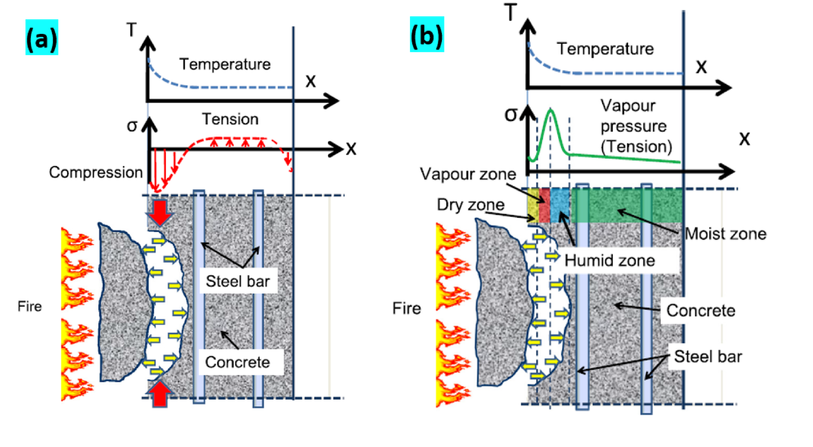
\includegraphics[width=0.7\linewidth]{figures/chapter2/spalling-mechanisms}
  \caption{Spalling combined mechanisms \cite{al-dalaien2025}}
  \label{fig:spalling-mechanisms}
\end{figure}

The spalling condition can be written schematically as:
\begin{equation}
    \sigma_{thermal}(T) + \sigma_{pore}(p_g,p_c,S_l) \ge f_t(T),
    \label{eq:spalling}
\end{equation}
where $\sigma_{thermal}$ is the thermal stress from differential dilation, $\sigma_{pore}$ the stress from pore-pressure loading, and $f_t(T)$ the temperature-degraded tensile strength. A comprehensive breakdown of this combined spalling mechanism is provided in \cref{sec:THM_spalling_app}.

\section{Improved thermo-hydro-chemical (THC) model} \label{sec:thcmodel}

\subsection{Motivation}
In standard Thermo-Hydric (TH) models, dehydration is treated through a fixed function of temperature alone - $\dot m_{dehyd}(T)$ and the porosity follows a simple linear law (as detailed in \cref{appendixA}). These simplifications overlook three facts that strongly affecting spalling:

\begin{enumerate}

\item The \emph{chemical state} of the cement paste before the accident depends on its hydration/curing history; 
\item The release of chemically bound water from the C--S--H is the chemical process that controls porosity, permeability and strength at high temperature; 
\item The chemical damage is essentially \emph{irreversible}. 

\end{enumerate} 
The improved Thermo-Hydro-Chemical (THC) model adopted here, following Scium\`e, Moreira and Dal~Pont \cite{sciume2024}, resolves the chemical field explicitly and couples it strictly to the thermal and hydric fields.

\subsection{Chemical state variables}
Unlike standard TH models, the THC framework explicitly resolves the chemical state of the cement paste. The evolution of the microstructure depends on two main processes \cite{sciume2024}:
\begin{itemize}
    \item \textbf{Hydration degree $\Gamma(t) \in [1]$:} Defines the formation of Calcium-Silicate-Hydrates (C-S-H) during curing and aging. Its evolution is governed by an Arrhenius-type chemo-kinetic law (detailed in \cref{sec:affinity}), driven by time, temperature, and relative humidity.
    \item \textbf{Dehydration degree $F(T) \in [1]$:} Represents the irreversible release of chemically bound water at high temperatures (typically $T > 105^\circ\mathrm{C}$).
\end{itemize}
To couple these effects, the \textbf{effective hydration degree} $\tilde{\Gamma}$ is introduced as the primary internal variable describing the state of the solid matrix:
\begin{equation}
    \tilde{\Gamma} = (1 - F(T))\,\Gamma
    \label{eq:effective-hydration}
\end{equation}
The transport and mechanical properties, such as porosity $\phi(\tilde{\Gamma})$ and intrinsic permeability $K(\tilde{\Gamma})$, are explicitly updated as functions of this effective hydration state. The specific evolution laws for these microstructural properties are detailed in \cref{sec:chemical_microstructure}.

\subsection{Resulting coupled system}
The standard Thermo-Hydric (TH) conservation equations for dry air, water species, and energy are detailed in \cref{eq:dry_air,eq:water_species,eq:energy_TH} of \cref{appendixA}. In these conventional formulations, the microstructural and chemical changes (e.g., the dehydration mass source $\dot{m}_{dehyd}$ and the porosity evolution) are treated implicitly via empirical functions of temperature alone.

By incorporating Powers' stoichiometry and the chemical couplings through the effective hydration degree $\tilde{\Gamma}$, the original system is profoundly transformed. The empirical functions are completely replaced by explicit chemo-physical interactions, reducing the final system to three highly non-linear conservation equations for the state variables $(p_g, p_c, T)$:

\paragraph{1. Dry-air conservation:}
\begin{equation}
    \underbrace{\frac{\partial}{\partial t}\big(\phi(1-S_l)\rho_a\big)}_{\text{Storage}} + \underbrace{\nabla \cdot (\mathbf{J}_a)}_{\text{Advection \& Diffusion}} = \underbrace{(1 - S_l)\rho_a \left(a_\phi \Omega \frac{\partial \tilde{\Gamma}}{\partial t}\right)}_{\text{Chemical coupling (porosity evolution)}}
\end{equation}

\paragraph{2. Total water-species conservation:}
\begin{equation}
    \underbrace{\frac{\partial}{\partial t}\big(\phi S_l \rho_l + \phi(1-S_l)\rho_v\big)}_{\text{Storage (Liquid + Vapor)}} + \underbrace{\nabla \cdot (\mathbf{J}_l + \mathbf{J}_v)}_{\text{Advection \& Diffusion}} = \underbrace{\left[ S_l\rho_l + (1-S_l)\rho_v \right] \left( a_\phi \Omega \frac{\partial \tilde{\Gamma}}{\partial t} \right)}_{\text{Porosity evolution}} - \underbrace{0.228 c \xi_\infty \frac{\partial \tilde{\Gamma}}{\partial t}}_{\text{De/hydration water source}}
\end{equation}

\paragraph{3. Energy conservation:}
\begin{equation}
    \underbrace{\overline{\rho C_p}\frac{\partial T}{\partial t}}_{\text{Heat storage}} + \underbrace{\mathbf{J}_{energy}^{adv}}_{\text{Advective heat flux}} - \underbrace{\nabla \cdot (\lambda \nabla T)}_{\text{Conduction}} = \underbrace{-H_{vap}\dot{m}_{vap}}_{\text{Phase change (Evaporation)}} + \underbrace{\left(H_{vap} 0.228 c \xi_\infty + L_{hyd}\right) \frac{\partial \tilde{\Gamma}}{\partial t}}_{\text{De/hydration latent heat}}
\end{equation}
where $a_\phi$ is the porosity evolution parameter, $c$ is the cement content, and $\xi_\infty$ is the maximum hydration fraction. The explicit formulation of these stoichiometric constants (e.g., the bound water $0.228 c \xi_\infty$ and the latent heat $L_{hyd}$) as well as the thermal activation energy $E_a/R$ governing $\tilde{\Gamma}$ are detailed in \cref{sec:powers} and \cref{sec:affinity} of \cref{appendixA}.

\section{Coupling to the mechanical field} \label{sec:mech}
The mechanical response is driven by the converged TH/THC fields through a \emph{one-way} (staggered) coupling: at each time step, the fields $(T,p_g,p_c)$ enter the mechanical problem as prescribed loading, and the resulting damage $\mathcal{D}$ feeds back weakly to the transport properties via permeability evolution at the next step. The TH/THC fields act through two routes:
\begin{itemize}
    \item \textbf{Free strains.} The total strain is decomposed as $\boldsymbol{\varepsilon}=\boldsymbol{\varepsilon}_\sigma+\boldsymbol{\varepsilon}_{th}+\boldsymbol{\varepsilon}_{sh}$, where $\boldsymbol{\varepsilon}_{th}$ is the thermal dilation (driven by $T$) and $\boldsymbol{\varepsilon}_{sh}$ the capillary shrinkage (driven by $p_c$). Creep is neglected, so $\boldsymbol{\varepsilon}_\sigma=\boldsymbol{\varepsilon}_{el}$.
    \item \textbf{Pore-pressure loading.} Through Bishop's effective stress $\boldsymbol{\sigma}'=\boldsymbol{\sigma}^{Total}+\alpha\,p_s\,\mathbf{I}$, the average pore pressure $p_s=p_g-S_l p_c$ enters the load vector as an external loading; its build-up shifts $\boldsymbol{\sigma}'$ towards tension and promotes cracking when $f_t(T)$ is exceeded.
\end{itemize}
Together with the spalling criterion \eqref{eq:spalling}, this closes the physical loop between the transport and mechanical fields. The mechanical constitutive model, its fracture-energy regularisation, and the spatial/temporal discretisation of the coupled problem are reported in full in \cref{appendixA}. 

\textbf{Note on the scope of the study:} Due to the limited timeframe of the internship and the fact that the experimental data used for validation (Kalifa test) solely provide temperature and gas pressure measurements, the mechanical module cannot be rigorously validated. Therefore, while this staggered mechanical coupling is mathematically formulated and designed as an easily pluggable module, the actual numerical simulations performed in the subsequent chapters are restricted to the TH(C) model.


% Chapter 3: Numerical implementation in Cast3M
\cleardoublepage
\chapter{Numerical implementation}

\review{This chapter is currently empty and is intended to outline the proposed structure of the thesis.}

As described by the governing equations in \cref{chapter2}, the numerical implementation in Cast3M is performed by solving the thermal, hydric, and mechanical models separately, and then coupling them together to form the THM coupled model. The implementation of each model and the coupling strategies are detailed in the following sections.

\section{Modeling strategy and model parameters}

\subsection{Modeling strategy}
This section is currently under development and will be refined as the study progresses.

\subsection{Geometry}
This section is currently under development and will be refined as the study progresses.

\begin{cast3m}
OPTI ECHO 0;
OPTI 'DIME' 2 'ELEM' 'QUA4' ;    

* 1) GEOMETRY AND MESH DEFINITION

*GEOMETRY DEFINITION
LONG    = 3.;
HAUT    = 0.5;

*NUMBER OF MESH SEGMENT
NLONG   = 35;
NHAUT   = 5;

*POINTS CREATION
PA      = 0. 0.;
PB      = LONG 0.;
PC      = LONG HAUT;
PD      = 0. HAUT;
TRAC (PA ET PB ET PC ET PD);

*MESH LINES CREATION
LAB     = DROI NLONG PA PB;
LBC     = DROI NHAUT PB PC;
LCD     = DROI NLONG PC PD;
LDA     = DROI NHAUT PD PA;

*MESH SURFACE CREATION
MAIL1   = DALL LAB LBC LCD LDA;
TRAC MAIL1;
\end{cast3m}


\subsection{Material properties}
\begin{reviewblock}
High-strength concrete with $f_{c,28} = 77$ MPa is adopted, and 18 key parameters are selected for sensitivity analysis \cite{liu2001}.
\end{reviewblock}

\subsection{Boundary conditions and loadings}
This section is currently under development and will be refined as the study progresses.

\section{Implementation of the thermal model}
\subsection{Stationary linear thermal analysis}
This section is currently under development and will be refined as the study progresses.
\subsection{Transient linear and non-linear thermal analysis}
This section is currently under development and will be refined as the study progresses.

\section{Implementation of the hydric model}
\subsection{Drying}
This section is currently under development and will be refined as the study progresses.
\subsection{Shrinkage}
This section is currently under development and will be refined as the study progresses.

\section{Implementation of the mechanical model}
\subsection{Elastic linear mechanical model}
This section is currently under development and will be refined as the study progresses.
\subsection{Mazars model}
This section is currently under development and will be refined as the study progresses.

\section{Implementation of the THM coupled model}
\subsection{TH coupling strategy}
This section is currently under development and will be refined as the study progresses.
\subsection{TM coupling strategy}
This section is currently under development and will be refined as the study progresses.
\subsection{THM coupling strategy}
This section is currently under development and will be refined as the study progresses.

\section{Integration into THM-D Coupled model}
This section is currently under development and will be refined as the study progresses.

\section{Numerical results}
This section is currently under development and will be refined as the study progresses.


% Chapter 4: Model validation and Experimental data
%\cleardoublepage %already included in mainmatter 
\chapter{Model Calibration and Validation} \label{chapter4}

\review{This chapter is currently empty and is intended to outline the proposed structure of the thesis.}
\section{Calibration procedure}

4.1 Calibration Strategy
Parameters investigated
Automation workflow (Python)
Calibration criteria
4.2 Results
Temperature evolution
Gas pressure evolution
Comparison with experimental data
4.3 Discussion
Influence of saturation degree
Influence of relative humidity
Model limitations

\section{Validation}
\subsection{Comparison between numerical and experimental results}
This section is currently under development and will be refined as the study progresses.
\subsection{Discussions on model performance}
This section is currently under development and will be refined as the study progresses.



% Chapter 5: Probabilistic sensitivity analysis
\cleardoublepage
\chapter{Probabilistic analysis of the THM model}

\review{This chapter is currently a draft version and will undergo further review and revision.}

\section{Sources of uncertainty and concrete heterogeneity}
This section follows the foundational framework presented in \cite{baroth2011}.

\begin{reviewblock}
Main ideas:
\begin{itemize}
  \item Concrete is not uniform, so its properties vary from place to place.
  \item Material parameters (e.g., stiffness and permeability) are uncertain.
  \item Measurements and model assumptions also add uncertainty.
\end{itemize}
\end{reviewblock}

\subsection{Motivation for probabilistic assessment}

In civil engineering, a structure or mechanical system is considered safe when it remains fit for duty for the duration of its service life, without causing damage to itself or its environment. Traditionally, deterministic models have been used to evaluate structural safety. However, the inevitable gap between a real physical system and a simplified numerical model, along with the unforeseeable nature of future loads and environmental conditions, inherently leads to uncertainty. 

To properly manage these risks and optimize the total lifecycle cost, modern engineering codes—such as the Eurocodes—rely heavily on probabilistic and statistical tools. The primary motivation for probabilistic assessment lies in its ability to explicitly quantify the safety of a structure through its probability of failure ($P_f$) and, conversely, its overall reliability ($R = 1 - P_f$). By adopting a probabilistic format, it becomes much easier to introduce random variables into mechanical behavior models, propagate them through structural analyses, and eventually make objective decisions based on both the probability of an event and the gravity of its consequences.

\subsection{Classification of uncertainties}

Predicting the exact lifetime or mechanical response of a construction project is impossible without accounting for multiple sources of uncertainty. According to reliability theory, these uncertainties can be broadly classified into two main categories: Aleatoric and Epistemic.

\begin{itemize}
    \item \textbf{Aleatoric (inherent or natural) uncertainties:} These uncertainties arise from the natural randomness of the environment and the spatial or temporal variability of material properties. Because they represent the inherent physical variation in nature, aleatoric uncertainties cannot be reduced or eliminated; they can only be accurately quantified (through data acquisition) and taken into account during the design process.
    
    \item \textbf{Epistemic (knowledge-based) uncertainties:} These stem from a lack of complete knowledge or insufficient data. They include \textit{model uncertainties} (the discrepancy between empirical or theoretical mathematical models and actual physical processes) and \textit{statistical uncertainties} (arising from limited data sampling or poor data collection methods). Furthermore, observation errors heavily contribute to epistemic uncertainty. These errors include measurement inaccuracies (caused by operators or poorly calibrated devices), representativity issues (e.g., deducing stress or rigidity indirectly from strain measurements), and time discrepancies (e.g., changes in material properties between the time of measurement and actual casting). Unlike aleatoric uncertainties, epistemic uncertainties can be effectively reduced by improving physical models, increasing training, and gathering more accurate data.
\end{itemize}

\subsection{Concrete heterogeneity and material variability}

A critical source of aleatoric uncertainty in civil engineering is the inherent heterogeneity of construction materials, such as concrete and geomaterials. 

\begin{itemize}
    \item \textbf{Historical and environmental dependence:} Concrete is not perfectly uniform. Its physical and mechanical properties depend heavily on its entire formation history, the conditions during casting, internal chemical reactions (like alkali-silica reactions), and long-term degradation processes caused by the surrounding environment.
    
    \item \textbf{Continuous and discrete spatial variations:} Because of this historical dependence, material parameters vary significantly from place to place. This spatial heterogeneity manifests in two ways:
    \begin{enumerate}
        \item \textit{Continuous variations:} Gradual spatial fluctuations in properties such as stiffness, Young's modulus, Poisson's ratio, density, or friction.
        \item \textit{Discrete variations:} The localized appearances of defects such as micro-cracks, water inlets, networks of capillaries, or weak points within the structure.
    \end{enumerate}
\end{itemize}

Because these material parameters are fundamentally variable, evaluating the true safety and performance of a structure requires geotechnical and structural predictions to abandon purely deterministic values. Instead, they must rely on random variables and stochastic fields to accurately model this spatial heterogeneity.

\section{Stochastic finite element framework} \label{sec:stochastic-framework}
In structural engineering, material properties such as the Young's modulus, permeability, or thermal conductivity are never perfectly known.
As noted by \cite{delarrard2010}, even under strict quality control the compressive strength of high-performance concrete can range from 62 to~100~MPa, reflecting the heterogeneous microstructure, cement composition, and environmental conditions during curing.
A \emph{deterministic} analysis assigns a single fixed value to each parameter and produces a unique structural response; it cannot, by itself, quantify the likelihood that a design limit will be exceeded.
A \emph{stochastic} (probabilistic) analysis, on the other hand, treats uncertain parameters as random quantities, propagates this uncertainty through the model, and delivers statistical information---mean, variance, probability of failure---about the structural response.

Two levels of stochastic description are used in this work. When a material property is spatially uniform but uncertain in magnitude, it is represented by a \emph{random variable} (\cref{subsec:random-variables}): a single uncertain value applies to the entire domain. When the property varies from point to point across the structure, it must be represented by a \emph{random field} (\cref{subsec:random-fields}): a spatially varying uncertain value is associated with every location, subject to a spatial correlation structure.
These two mathematical objects form the theoretical foundation for the Gaussian Quadrature method (\cref{sec:quadrature}) and the Monte Carlo simulation (\cref{sec:monte-carlo}), respectively.


\subsection{Random variables (PDF, CDF, moments, CoV)}

\review{This section is currently under development and will be refined as the study progresses.}

A \textbf{random variable} $X$ is a quantity whose value is not fixed but described by a probability law.
Instead of saying ``$E = 30$~GPa'', one writes $E \sim \mathcal{N}(30,\,3^2)$~GPa, meaning that the Young's modulus follows a normal (Gaussian) distribution with mean $\mu = 30$~GPa and standard deviation $\sigma = 3$~GPa.

\subsubsection{Probability Density Function (PDF)}

The \textbf{probability density function} (PDF) $f_X(x)$ characterises the likelihood of $X$ taking a given value. It satisfies:

\begin{draftblock}

\begin{equation}
    f_X(x) \geq 0 \quad \forall\, x, \qquad
    \int_{-\infty}^{+\infty} f_X(x)\,\mathrm{d}x = 1.
    \label{eq:pdf-properties}
\end{equation}

For a \textbf{normal} (Gaussian) distribution $\mathcal{N}(\mu,\sigma^2)$:

\begin{equation}
    f_X(x) = \frac{1}{\sigma\sqrt{2\pi}}\,
    \exp\!\left[-\frac{(x-\mu)^2}{2\sigma^2}\right].
    \label{eq:pdf-normal}
\end{equation}

For a \textbf{lognormal} distribution $\mathrm{LN}(\mu_{\ln},\sigma_{\ln}^2)$, the variable $\ln X$ is normally distributed, ensuring $X > 0$:

\begin{equation}
    f_X(x) = \frac{1}{x\,\sigma_{\ln}\sqrt{2\pi}}\,
    \exp\!\left[-\frac{(\ln x - \mu_{\ln})^2}{2\sigma_{\ln}^2}\right],
    \qquad x > 0.
    \label{eq:pdf-lognormal}
\end{equation}

The lognormal distribution is particularly relevant for material properties such as the Young's modulus or permeability, which must remain strictly positive \cite{delarrard2010,sudret2000}.

\end{draftblock}

\subsubsection{Cumulative Distribution Function (CDF)}

The \textbf{cumulative distribution function} (CDF) $F_X(x)$ gives the probability that $X$ does not exceed a threshold:

\begin{draftblock}

\begin{equation}
    F_X(x) = P(X \leq x) = \int_{-\infty}^{x} f_X(t)\,\mathrm{d}t.
    \label{eq:cdf-def}
\end{equation}

$F_X$ is a non-decreasing function with $F_X(-\infty) = 0$ and $F_X(+\infty) = 1$.
In reliability analysis, the CDF is used directly to evaluate the probability of exceeding a critical value: $P(X > x_{\mathrm{cr}}) = 1 - F_X(x_{\mathrm{cr}})$.

\end{draftblock}

\subsubsection{Statistical moments}

The distribution of $X$ can be summarised by its \textbf{statistical moments}, which quantify location, spread, asymmetry, and tail heaviness:

\begin{enumerate}
    \item \textbf{Mean} (first moment, expected value):
    
    \begin{equation}
        \mu_X = E[X] = \int_{-\infty}^{+\infty} x\, f_X(x)\,\mathrm{d}x.
        \label{eq:mean}
    \end{equation}

    \item \textbf{Variance} (second central moment):
    
    \begin{equation}
        \sigma_X^2 = \mathrm{Var}[X] = E\!\left[(X - \mu_X)^2\right]
        = \int_{-\infty}^{+\infty} (x - \mu_X)^2\, f_X(x)\,\mathrm{d}x.
        \label{eq:variance}
    \end{equation}
    
    The \textbf{standard deviation} $\sigma_X = \sqrt{\mathrm{Var}[X]}$ has the same unit as $X$.

    \item \textbf{Skewness} (third standardised moment):
    
    \begin{equation}
        \gamma_3 = \frac{E\!\left[(X - \mu_X)^3\right]}{\sigma_X^3}.
        \label{eq:skewness}
    \end{equation}
    
    $\gamma_3 = 0$ for a symmetric distribution (e.g.\ Gaussian); $\gamma_3 > 0$ indicates a right-skewed distribution (e.g.\ lognormal).

    \item \textbf{Kurtosis} (fourth standardised moment):
    
    \begin{equation}
        \gamma_4 = \frac{E\!\left[(X - \mu_X)^4\right]}{\sigma_X^4}.
        \label{eq:kurtosis}
    \end{equation}
    
    $\gamma_4 = 3$ for the Gaussian distribution.
    Heavy-tailed distributions have $\gamma_4 > 3$.
\end{enumerate}

These four moments play a central role in the Gaussian Quadrature method (\cref{sec:quadrature}), where the response PDF is reconstructed from the computed moments using Winterstein or Pearson approximations \cite{sudret2003}.

\subsubsection{Coefficient of Variation (CoV)}

The \textbf{coefficient of variation} quantifies the relative dispersion of $X$:

\begin{equation}
    \mathrm{CoV}_X = \frac{\sigma_X}{\mu_X}.
    \label{eq:cov}
\end{equation}

It is a dimensionless measure that allows comparison of variability across parameters with different units and magnitudes.
For concrete, typical values are $\mathrm{CoV}_E \approx 0.10$--$0.20$ for the Young's modulus \cite{delarrard2010} and $\mathrm{CoV}_K \approx 0.15$--$0.30$ for permeability.


\subsection{Random fields and correlation structure}

\review{This section is currently under development and will be refined as the study progresses.}

\subsubsection{Random fields}

A random variable assigns a \emph{single} uncertain value to a material property for the entire structure. In reality, concrete properties vary spatially due to heterogeneous microstructure, local variations in the water-to-cement ratio, and non-uniform compaction duringcasting \cite{delarrard2010}.
A \textbf{random field} extends the notion of a random variable to continuous space: it associates an uncertain value with \emph{every point} $\mathbf{x}$ in the structural domain $\mathcal{D} \subset \mathbb{R}^d$.

\begin{draftblock}
    
A random field is a collection of random variables indexed by position:

\begin{equation}
    H \;=\; \bigl\{H(\mathbf{x},\omega) : \mathbf{x} \in \mathcal{D},\;
                                            \omega \in \Omega \bigr\},
    \label{eq:rf-definition}
\end{equation}

where $\omega$ denotes a particular realisation (outcome) drawn from the probability space $(\Omega, \mathcal{F}, P)$ \cite{sudret2000}. For a fixed $\omega$, $H(\cdot,\omega)$ is a deterministic spatial function called a \emph{realisation} of the random field; for a fixed $\mathbf{x}$, $H(\mathbf{x},\cdot)$ is an ordinary random variable.

A second-order random field is fully characterised by two functions \cite{sudret2000}:
\begin{itemize}
    \item the \textbf{mean field}:
    \begin{equation}
        \bar{H}(\mathbf{x}) \;=\; E\!\left[H(\mathbf{x},\omega)\right],
        \label{eq:rf-mean}
    \end{equation}
    \item the \textbf{covariance function}:
    \begin{equation}
        C_H(\mathbf{x},\mathbf{y})
        \;=\; E\!\left[
            \bigl(H(\mathbf{x}) - \bar{H}(\mathbf{x})\bigr)
            \bigl(H(\mathbf{y}) - \bar{H}(\mathbf{y})\bigr)
        \right].
        \label{eq:rf-covariance}
    \end{equation}
\end{itemize}

The covariance function quantifies the statistical dependence between the values of $H$ at two distinct locations. A random field is called \textbf{homogeneous} (or \emph{stationary}) if both $\bar{H}(\mathbf{x})$ and $C_H(\mathbf{x},\mathbf{y})$ depend only on the separation vector $\boldsymbol{\tau} = \mathbf{x} - \mathbf{y}$, i.e.$C_H(\mathbf{x},\mathbf{y}) = C_H(\boldsymbol{\tau})$.

\end{draftblock}

\subsubsection{Correlation function and correlation length} \label{sec:correlation}

For a homogeneous random field, the \textbf{autocorrelation function} $\rho_H(\boldsymbol{\tau})$ is defined by normalising the covariance:

\begin{draftblock}

\begin{equation}
    \rho_H(\boldsymbol{\tau})
    \;=\; \frac{C_H(\boldsymbol{\tau})}{\sigma_H^2},
    \qquad \rho_H(\mathbf{0}) = 1,
    \label{eq:autocorrelation}
\end{equation}

where $\sigma_H^2 = C_H(\mathbf{0})$ is the variance of the field. The most common model for concrete material properties is the \textbf{squared-exponential} (Gaussian) correlation function \cite{sudret2000,fenton2014}:

\begin{equation}
    \rho_H(\tau) \;=\; \exp\!\left(-\frac{\tau^2}{L_c^2}\right),
    \label{eq:corr-gaussian}
\end{equation}

and the \textbf{exponential} (Markov) correlation function:

\begin{equation}
    \rho_H(\tau) \;=\; \exp\!\left(-\frac{|\tau|}{L_c}\right),
    \label{eq:corr-exponential}
\end{equation}

where $\tau = \|\boldsymbol{\tau}\|$ is the Euclidean distance between two points, and $L_c > 0$ is the \textbf{correlation length}.

\end{draftblock}

The correlation length $L_c$ is the central parameter of the random field model. It controls the spatial scale over which the field exhibits coherent variations:

\begin{itemize}
    \item If $L_c \gg L_{\mathrm{struct}}$ (the structural dimension), the field is nearly uniform in space and behaves like a random variable: one realisation has almost the same value everywhere.
    \item If $L_c \ll L_{\mathrm{struct}}$, adjacent points are nearly independent and the field fluctuates rapidly over short distances.
    \item For intermediate values, the field exhibits smooth but spatially varying realisations, which is the typical case for concrete \cite{delarrard2010}.
\end{itemize}

The effect of $L_c$ on structural response is illustrated in \cref{fig:correlation-length-effect}: a small $L_c$ produces highly heterogeneous fields that may create local weak zones, whereas a large $L_c$ produces fields closer to a uniform random variable.

\subsection{Summary: random variable versus random field}

\cref{tab:rv-vs-rf} summarises the key differences between the two levels of stochastic description and their implications for the numerical methods used in this work.

\begin{table}[htbp]
\centering
\caption{Comparison of random variable and random field stochastic descriptions.}
\label{tab:rv-vs-rf}
\begin{tabular}{p{4cm} p{4.5cm} p{4.5cm}}
\textbf{Aspect}
    & \textbf{Random variable}
    & \textbf{Random field} \\
Spatial variation
    & None (spatially uniform)
    & Yes (spatially heterogeneous) \\[4pt]
Characterisation
    & PDF: mean $\mu$, std $\sigma$
    & Mean field $\bar{H}(\mathbf{x})$, covariance $C_H(\mathbf{x},\mathbf{y})$ \\[4pt]
Key parameter
    & CoV
    & Correlation length $L_c$ \\[4pt]
Stochastic level
    & First-order
    & Second-order \\[4pt]
Resolution method
    & Gaussian Quadrature
    & Karhunen--Lo\`eve + Monte Carlo \\[4pt]
Cast3m operator
    & \texttt{QUADRATU}
    & \texttt{ALEA} \\[4pt]
Computational cost
    & Low (3--7 runs per variable)
    & High (hundreds to thousands of runs) \\
\end{tabular}
\end{table}

The choice between these two levels of description is governed by the spatial scale of heterogeneity relative to the structural dimensions. For the THM analyses presented in this work, the Gaussian Quadrature method (\cref{sec:quadrature}) is applied when properties are treated as spatially uniform uncertain quantities, while the Monte Carlo method (\cref{sec:monte-carlo}) is employed when spatial variability is explicitly modelled.

\section{Monte Carlo simulation framework} \label{sec:monte-carlo}

Monte Carlo simulation (MCS) is the reference method for propagating uncertainty through complex nonlinear models such as the THM framework adopted in this work. Its principle is straightforward: a large number of independent realisations of the uncertain input fields are generated, the deterministic model is evaluated for each realisation, and theresulting ensemble of responses is used to estimate statistics and failure probabilities \cite{fenton2014}. Because no assumption is made on the shape of the response surface, MCS is able to estimate the \emph{entire} output distribution, a major advantage over linearisation methods such as FORM/SORM \cite{fenton2014}.

\subsection{Principle and convergence}

\review{This section is currently under development and will be refined as the study progresses.}

\begin{draftblock}

\paragraph{General procedure}

Each Monte Carlo trial consists of three steps \cite{fenton2014}:

\begin{enumerate}
    \item Generate a realisation of the random input (random variable or random field) according to its prescribed distribution.
    \item Evaluate the deterministic model (here, the THM finite element solver in Cast3M) to obtain the system response.
    \item Repeat steps 1--2 until the output statistics have converged to a stable estimate.
\end{enumerate}

The probability of failure $p_f$ is estimated as:

\begin{equation}
    \hat{p}_f = \frac{N_f}{n},
    \label{eq:mc-pf}
\end{equation}

where $N_f$ is the number of realisations for which the limit state function $g < 0$ (failure), and $n$ is the total number of realisations. Since $N_f$ follows a binomial distribution, $\hat{p}_f$ is an unbiased estimator of $p_f$ \cite{fenton2014}.

\paragraph{Convergence criterion}

The variance of the estimator $\hat{p}_f$ is:

\begin{equation}
    \mathrm{Var}[\hat{p}_f] = \frac{p_f(1-p_f)}{n},
    \label{eq:mc-variance}
\end{equation}

so that the standard deviation of the estimate decreases as $1/\sqrt{n}$. For a maximum tolerable absolute error $e$ at $95\%$ confidence level, the required number of realisations is \cite{fenton2014}:

\begin{equation}
    n \;\geq\; \frac{4\,p_f(1-p_f)}{e^2}.
    \label{eq:mc-nsample}
\end{equation}

For example, estimating $p_f \approx 10^{-3}$ with a relative error of $10\%$ (i.e.\ $e = 10^{-4}$) at $95\%$ confidence requires $n \approx 400{,}000$ realisations \cite{fenton2014}. This illustrates the main limitation of crude MCS for rare-event estimation: the computational cost grows rapidly as $p_f$ decreases. In the context of THM finite element analyses, where a single evaluation may take several minutes, this cost is prohibitive and motivates the use of the Gaussian Quadrature method presented in
\cref{sec:quadrature}.

\paragraph{Convergence in practice}

When highly accurate probability estimates for low-probability events are not achievable directly, two complementary strategies are employed \cite{fenton2014}:

\begin{itemize}
    \item \textbf{Distribution fitting}: fit a parametric distribution to the simulated response and extrapolate into the tails. This is justified by the central limit theorem when the response is approximately a sum or product of independent contributions.
    \item \textbf{Variance reduction}: use simulation techniques such as antithetic variates (negatively correlated pairs) to reduce the variance of the estimator for a given $n$.
\end{itemize}
    
\end{draftblock}

\subsection{Transformation of Lognormal to Gaussian distribution} \label{sec:lognormal-transformation}

In practical finite element implementations using the Cast3M software, material parameters such as Young's modulus and permeability must remain strictly positive. However, the built-in random field operator \texttt{ALEA} generates Gaussian (normal) distributions, necessitating a mathematical transformation \cite{sudret2000}.

A \textbf{lognormal random field} $H(\mathbf{x})$ is therefore adopted: by definition, $\ln H(\mathbf{x})$ is a Gaussian random field, which guarantees $H(\mathbf{x}) > 0$ at every point \cite{delarrard2010}. The moments of $H(\mathbf{x})$ are related to those of the underlying Gaussian field $G(\mathbf{x}) \sim \mathcal{N}(\mu_{\ln},\,\sigma_{\ln}^2)$ by \cite{sudret2000}:

\begin{equation}
    \begin{cases}
        \mu_X \;=\; \exp\!\left(\mu_{\ln} + \dfrac{\sigma_{\ln}^2}{2}\right) \\[8pt]
        \sigma_X^2 \;=\; \left[\exp(\sigma_{\ln}^2) - 1\right]
                         \exp\!\left(2\mu_{\ln} + \sigma_{\ln}^2\right)
    \end{cases}
    \label{eq:lognormal-system}
\end{equation}

where $\mu_X$ and $\sigma_X$ are the physical mean and standard deviation of the material property. Inverting \cref{eq:lognormal-system} yields the Gaussian parameters as functions of the physical moments:

\begin{equation}
    \sigma_{\ln}^2 = \ln\!\left(1 + CoV_X^2\right),
    \qquad
    \mu_{\ln} = \ln(\mu_X) - \tfrac{1}{2}\,\sigma_{\ln}^2,
    \label{eq:lognormal-params}
\end{equation}

where $CoV_X = \sigma_X/\mu_X$ is the coefficient of variation.

The standard computational procedure in Cast3M \texttt{ALEA} then consists of two steps:

\begin{enumerate}
    \item Generate a Gaussian random field
          $G(\mathbf{x}) \sim \mathcal{N}(\mu_{\ln},\,\sigma_{\ln}^2)$ using the Turning Band Method (see \cref{sec:tbm}), with parameters computed from \cref{eq:lognormal-params}.

    \item Transform pointwise to obtain the lognormal field:
          \begin{equation}
              H(\mathbf{x}) \;=\;
              \exp\!\bigl(G(\mathbf{x})\bigr),
              \label{eq:lognormal-transform}
          \end{equation}
          which guarantees $H(\mathbf{x}) > 0$ and preserves the correlation structure characterised by $L_c$ (see \cref{sec:correlation}).
\end{enumerate}

This pointwise transformation is exact: the autocorrelation structure of the underlying Gaussian field is preserved in the lognormal field, so the spatial variability characterised by the correlation length $L_c$ remains physically meaningful after transformation \cite{delarrard2010}.

\subsection{Random field generation and discretization}
Representing the spatial variability of material properties in a finite element model requires both a method to \emph{generate} a random field realisation over the domain and a strategy to \emph{discretise} it onto the mesh, so that spatially varying values can be assigned directly to the elements or integration points of the finite element model. Several approaches exist in the literature; the principal families are surveyed below before the Turning Bands Method adopted in this work is described in detail in \cref{sec:tbm}.

\subsubsection{Overview of generation methods} \label{sec:rf-methods}
A random field $H(\mathbf{x}, \omega)$ with prescribed mean, variance, and covariance structure $C(\mathbf{x}, \mathbf{x}')$ can be simulated by several families of methods \cite{fenton2014}:

\begin{itemize}
    \item \textbf{Matrix decomposition (Cholesky).}
          The covariance matrix $\mathbf{C}$ is factorised as $\mathbf{C} = \mathbf{L}\mathbf{L}^T$ and a correlated realisation is obtained as $\mathbf{h} = \mathbf{L}\mathbf{z}$, where $\mathbf{z}$ is a vector of independent standard normal variates \cite{fenton2014}. The method is exact but scales as $\mathcal{O}(n^3)$ in the number of nodes $n$, making it prohibitive for large meshes.

    \item \textbf{Spectral methods (FFT-based).}
          Realisations are generated by filtering white noise in the frequency domain using the spectral density corresponding to the target covariance \cite{fenton2014}. FFT algorithms are computationally efficient on regular grids, but the method is limited to stationary fields on rectangular domains with periodic boundary conditions.
    \item \textbf{Local Average Subdivision (LAS).}
          LAS generates the random field by successively subdividing the domain and assigning local averages consistent with the target covariance at each level of refinement \cite{fenton2014}. The method is computationally efficient and naturally produces spatially averaged values over elements, making it well-suited for direct use in finite element models. However, it is primarily designed for regular rectangular grids.

    \item \textbf{Series expansion methods.}
          Methods such as the Karhunen--Loève (KL) expansion parametrise the random field as a finite series of deterministic spatial functions multiplied by independent random variables \cite{sudret2000, delarrard2010}. They provide a compact representation of the spatial variability but require solving a global eigenvalue problem on the finite element mesh, whose cost increases with mesh size and targeted accuracy.

    \item \textbf{Turning Bands Method (TBM).}
          The TBM reduces the $d$-dimensional simulation to a set of one-dimensional stationary processes along random lines (bands) passing through the domain \cite{matheron1973, fenton2014}. It requires neither a global matrix factorisation nor an eigenvalue solve, and operates directly on any mesh geometry. The method is described in detail in \cref{sec:tbm} and is the approach adopted in this work.

\end{itemize}

\subsubsection{Turning Bands Method for random field generation} \label{sec:tbm}
\paragraph{Principle}

The Turning Bands Method (TBM), introduced by \cite{matheron1973}, generates a random field over a 2-D or 3-D domain by combining a set of simple 1-D random processes. The idea is illustrated in \cref{fig:tbm}: a number $L$ of lines (bands) are drawn through the domain in uniformly distributed directions. Along each line, an independent 1-D random process is simulated. The value of the field at any point $\mathbf{x}$ is then obtained by projecting that point onto each line and averaging the 1-D values:

\begin{equation}
    Z(\mathbf{x}) \;=\; \frac{1}{\sqrt{L}}
    \sum_{i=1}^{L}
    Z_i\!\left(\mathbf{x} \cdot \mathbf{u}_i\right),
    \label{eq:tbm}
\end{equation}

where $\mathbf{u}_i$ is the unit direction vector of the $i$-th band and $Z_i$ is the corresponding 1-D process. The 1-D processes are constructed so that the resulting 2-D field reproduces the prescribed spatial covariance structure, for instance the isotropic exponential model:

\begin{equation}
    C(\mathbf{x}, \mathbf{x}') \;=\;
    \sigma^2 \exp\!\left(
        -\frac{\|\mathbf{x} - \mathbf{x}'\|}{L_c}
    \right),
    \label{eq:cov-expo}
\end{equation}

where $L_c$ is the correlation length, mentioned in \cref{sec:correlation} controlling how rapidly the field varies in space. The quality of the simulation improves with the number of bands; in practice $L = 16$ issufficient for isotropic fields in two dimensions \cite{fenton2014}.

\paragraph{Implementation in Cast3M}

The TBM is natively implemented in the Cast3M \texttt{ALEA} operator, which takes as input the Gaussian parameters $(\mu_{\ln}, \sigma_{\ln})$ and the correlation length $L_c$, and returns the simulated field directly as nodal values on the mesh. The lognormal transformation and assignment to \texttt{MATE} follow the procedure described in \cref{sec:lognormal-transformation}.

\subsection{Integration of spatial variability into the THM model} \label{sec:thm-integration-mc}
This section is currently under development and will be refined as the study progresses.

Once the lognormal random field $H(\mathbf{x})$ has been constructed via the Turning Band Method (see \cref{sec:tbm}), it is propagated through the nonlinear THM model using Monte Carlo simulation. Given the computational cost of each THM evaluation, the iterative procedure is fully automated in Cast3M using the \texttt{REPETER} operator.

\subsubsection{Simulation loop and dynamic material updating} \label{sec:mc-loop}

This section is currently under development and will be refined as the study progresses.

\begin{draftblock}

For a predefined number of simulations $N_{simu}$, the global algorithm performs the following sequential steps within each loop:

\begin{enumerate}
    \item \textbf{Random Field Generation:} A new statistically independent realization of the random field is generated using the \texttt{ALEA} operator. For instance, the spatial distribution of the Young's modulus $\mathbf{E}(x)$ is recalculated based on the assigned log-normal parameters (mean, standard deviation, and correlation length).
    \item \textbf{Material Updating:} The macroscopic properties of the finite element model are updated. The newly generated random field is projected onto the mesh to form the updated material stiffness matrix using the \texttt{MATE} operator.
    \item \textbf{Non-linear Resolution:} The \texttt{PASAPAS} procedure is invoked to solve the multi-physics THM problem from $t=0$ to the final time $t_{fin}$, utilizing the updated heterogeneous material properties.
\end{enumerate}
\end{draftblock}

\subsubsection{Data extraction and post-processing}

This section is currently under development and will be refined as the study progresses

\begin{draftblock}
Storing the complete output database (which includes nodal displacements, stress tensors, and internal damage variables for every time step) for hundreds of simulations would result in an unmanageable amount of data and exceed memory limits. Therefore, a selective data extraction strategy is implemented.

Instead of saving the entire mesh history, a specific "Quantity of Interest" (QoI) is dynamically extracted at the end of each calculation loop. Depending on the targeted sensitivity analysis for the spalling risk, the QoI could be the maximum equivalent plastic strain, the peak pore pressure, or the maximum macroscopic damage variable $D$. 

In the Cast3M script, this is executed using the \texttt{EXCO} (to extract the specific component, e.g., the internal variable \texttt{'V1'} for damage) and \texttt{MAXI} operators to find the extreme value over the spatial domain. Finally, the extracted scalar values are continuously appended to an external structured text file (CSV format) using the \texttt{SORT 'CHAI'} command. 

This exported dataset containing the input realizations and the corresponding QoI outputs serves as the direct input for the external probabilistic software (e.g., Persalys) to compute the probability density functions and rank the dominant parameters via Sobol indices.
\end{draftblock}

\section{Gaussian Quadrature framework} \label{sec:quadrature}

The Gaussian Quadrature method offers a fundamentally different approach to uncertainty propagation compared to Monte Carlo simulation: instead of generating a large number of random realisations, it evaluates the THM model at a small, strategically chosen set of deterministic points and reconstructs the output statistics from a weighted sum \cite{Baldeweck1999, sudret2003}. This section describes the mathematical framework of the method, its application to moment and PDF estimation, and its integration into the Cast3M environment.

\subsection{Principle of Gaussian Quadrature}
\begin{draftblock}

Consider a scalar response quantity $G = g(\mathbf{X})$, where $\mathbf{X} = \{X_1, \ldots, X_N\}$ is a vector of independent random variables with joint PDF $f_{\mathbf{X}}(\mathbf{x})$. Computing any statistical moment of $G$ requires evaluating an integral of the form:

\begin{equation}
    I \;=\; \int_{\mathcal{D}} g(\mathbf{x})\, W(\mathbf{x})\,
    \mathrm{d}\mathbf{x},
    \label{eq:quad-integral}
\end{equation}

where $W(\mathbf{x}) = f_{\mathbf{X}}(\mathbf{x})$ plays the role of a weighting function \cite{sudret2003}. For a single random variable with weighting function $W(x)$, this integral is approximated by a weighted sum over $K$ strategically placed evaluation points (abscissas) $\{x_k\}$:

\begin{equation}
    I \;\approx\; \sum_{k=1}^{K} w_k\, g(x_k),
    \label{eq:quad-1d}
\end{equation}

where $\{w_k, x_k\}_{k=1}^K$ are the quadrature weights and abscissas associated with $W$ \cite{Baldeweck1999}.

The key result of Gaussian quadrature theory is that the optimal abscissas are the roots of the $K$-th order orthogonal polynomial $P_K$ with respect to the scalar product induced by $W$ \cite{sudret2003}:

\begin{equation}
    \langle f, g \rangle \;=\;
    \int_{\mathcal{D}} f(x)\, g(x)\, W(x)\, \mathrm{d}x.
    \label{eq:scalar-product}
\end{equation}

These polynomials $\{P_j\}$ are constructed by Gram-Schmidt orthogonalisation via the three-term recurrence:

\begin{equation}
    P_{j+1}(x) \;=\;
    (x - a_j)\,P_j(x) \;-\; b_j\,P_{j-1}(x),
    \quad j \geq 1,
    \label{eq:recurrence}
\end{equation}

with $P_0(x) = 1$ and $P_1(x) = x - a_0$, where $a_j$ and $b_j$ are scalar products of consecutive polynomials \cite{sudret2003}. The corresponding integration weights are given by:

\begin{equation}
    w_k \;=\;
    \frac{\langle P_{K-1},\, P_{K-1} \rangle}
         {P'_K(x_k)\, P_{K-1}(x_k)},
    \quad k = 1, \ldots, K,
    \label{eq:quad-weights}
\end{equation}

where $P'_K$ denotes the first derivative of $P_K$. A $K$-point scheme integrates exactly any polynomial function of degree up to $2K - 1$ \cite{sudret2003}.
    
\end{draftblock}

In Cast3M, the operator \texttt{QUADRATU} automatically computes the abscissas and weights for any prescribed distribution (Normal, Lognormal, Uniform, etc.) by applying the recurrence in \cref{eq:recurrence} with the appropriate weighting function. The user provides only the distribution type and its parameters; no manual derivation of quadrature points is required.

\subsection{Statistical moment estimation}

\begin{draftblock}
\paragraph{Multi-variable extension}

For a vector of $N$ independent random variables, the $q$-th moment of $G$ is a multiple integral over the joint domain:

\begin{equation}
    \mu_q^{(0)} \;=\;
    \int_{D_1 \times \cdots \times D_N}
    \bigl[g(x_1, \ldots, x_N)\bigr]^q\,
    f_1(x_1) \cdots f_N(x_N)\,
    \mathrm{d}x_1 \cdots \mathrm{d}x_N.
    \label{eq:moment-integral}
\end{equation}

Applying the 1-D quadrature rule \cref{eq:quad-1d} separately to each variable using $K_j$-point schemes yields the tensor-product approximation \cite{Baldeweck1999, sudret2003}:

\begin{equation}
    \mu_q^{(0)} \;\approx\;
    \sum_{k_1=1}^{K_1} \cdots \sum_{k_N=1}^{K_N}
    w_{k_1}^{(1)} \cdots w_{k_N}^{(N)}\,
    \bigl[g\bigl(x_{k_1}^{(1)}, \ldots, x_{k_N}^{(N)}\bigr)\bigr]^q.
    \label{eq:moment-quadrature}
\end{equation}

The central moments $\mu_q$ (variance, skewness, kurtosis) are computed similarly by replacing $[g(\cdot)]^q$ with $[g(\cdot) - \mu_1^{(0)}]^q$. In practice, the first four moments are computed: mean $\mu$, standard deviation $\sigma$, skewness $\delta_3 = \mu_3/\sigma^3$, and kurtosis $\delta_4 = \mu_4/\sigma^4$ \citp{sudret2003}.
\end{draftblock}

\paragraph{Output in Cast3M}

The operator \texttt{PARASTAT} collects the model evaluations at each quadrature point and assembles the weighted sums in \cref{eq:moment-quadrature}. The four moments are returned directly and can be inspected or used for subsequent PDF reconstruction and reliability assessment.

\subsection{PDF, CDF and reliability assessment}

\begin{draftblock}
    
\paragraph{PDF reconstruction from moments}

Once the first four moments $(\mu, \sigma, \delta_3, \delta_4)$
of $G$ are known, a continuous PDF $\tilde{f}_G$ is reconstructed
by fitting a parametric family to these moments. Three methods are
available in the Cast3M \texttt{PROBDENS} operator
\cite{sudret2003}:

\begin{itemize}
    \item \textbf{Winterstein approximation.} $G$ is expressed as
          a third-order Hermite polynomial transformation of a
          standard normal variable $\xi$:
          %
          \begin{equation}
              \tilde{G}(\xi) \;=\;
              \mu \;+\; \tilde{k}\sigma
              \bigl[\xi + h_3(\xi^2 - 1) + h_4(\xi^3 - 3\xi)\bigr],
              \label{eq:winterstein}
          \end{equation}
          %
          where the coefficients $\tilde{k}$, $h_3$, $h_4$ are
          determined by matching the four moments of $\tilde{G}$
          to those of $G$ \cite{sudret2003}. The CDF and PDF
          follow analytically from the standard normal CDF $\Phi$
          and PDF $\varphi$.

    \item \textbf{Pearson's method.} The PDF is assumed to satisfy
          a first-order ODE whose coefficients are expressed in
          terms of the four moments, yielding a family of
          distributions (normal, beta, gamma, Student, etc.)
          depending on the discriminant of the equation
          \cite{sudret2003}.

    \item \textbf{Exponential of polynomials.} The PDF is modelled
          as $\tilde{f}_G(\gamma) = c\,\exp(Q(\gamma))$, where
          $Q$ is a polynomial of degree $n$ ($n = 3$ to $6$)
          whose coefficients are fitted to the moments by solving
          a linear system \cite{sudret2003}.
\end{itemize}

All three methods yield consistent results in the central region
$[\mu - 3\sigma,\; \mu + 3\sigma]$; differences appear mainly in
the distribution tails \cite{sudret2003}.

\paragraph{Probability of failure and reliability index}

Once $\tilde{f}_G$ (or equivalently the CDF $\tilde{F}_G$) is
available, the probability of failure associated with the limit
state $\{G \leq 0\}$ is:
%
\begin{equation}
    P_f \;=\; \tilde{F}_G(0),
    \label{eq:pf}
\end{equation}
%
and the generalised reliability index is:
%
\begin{equation}
    \beta \;=\; -\Phi^{-1}(P_f).
    \label{eq:beta}
\end{equation}
%
The method provides accurate results for reliability indices
$\beta \lesssim 4$ to $5$ \cite{sudret2003}.

\end{draftblock}

\subsection{Integration and Computational efficiency}

\begin{reviewblock}
Main ideas as follows:
\end{reviewblock}

\subsubsection{Cost comparison with Monte Carlo}

\begin{draftblock}
The total number of model evaluations required by the
tensor-product quadrature scheme with $K$ points per variable
and $N$ random variables is:
%
\begin{equation}
    N_{\mathrm{eval}} \;=\; K^N.
    \label{eq:eval-count}
\end{equation}
%
For the THM model considered in this work with $N = 2$ uncertain
parameters (permeability $K_{\mathrm{int}}$ and Young modulus
$E$) and a 3-point scheme ($K = 3$), this gives
$3^2 = 9$ deterministic finite element runs — compared to
several thousand runs typically required for Monte Carlo
convergence. Each run is computationally expensive (a full
transient THM simulation); the reduction in cost by a factor
of $\mathcal{O}(10^2)$ to $\mathcal{O}(10^3)$ is therefore
practically decisive.
\end{draftblock}

\subsubsection{Quick Quadrature for high-dimensional problems}

\begin{draftblock}
    
When the number of random variables is larger, the full
tensor-product scheme becomes expensive. A \emph{quick
quadrature} variant can be used when two conditions are met:
(a) the model response values $g(\mathbf{x}_{k_1,\ldots,k_N})$
are of comparable magnitude across all quadrature points, and
(b) the combined weights $w_{k_1} \cdots w_{k_N}$ vary by
several orders of magnitude \cite{sudret2003}. In this case,
all $K^N$ weight products are sorted in descending order and
only the first $\tilde{K} \ll K^N$ terms whose cumulative sum
reaches $1 - \varepsilon$ are evaluated, where $\varepsilon$
is a user-prescribed tolerance. This reduces the number of
finite element runs significantly while maintaining a
prescribed accuracy level \cite{sudret2003}.

For the present study with $N = 2$, the full tensor-product
scheme is tractable and the quick quadrature option is not
required.
\end{draftblock}

\subsubsection{Data extraction: moments computed directly from weighted sum}

\begin{draftblock}
    
A by-product of the quadrature framework is the ability to
perform a global sensitivity analysis at negligible additional
cost. Since the model has already been evaluated at all
tensor-product quadrature points, the contribution of each
random variable $X_j$ to the total output variance can be
estimated by comparing the variance of the conditional mean
$\mathbb{E}[G \mid X_j]$ to the total variance $\mathrm{Var}(G)$
\cite{sudret2003}. In Cast3M, this is carried out by
\texttt{PARASTAT} using the Pearson correlation coefficients
between each input and the output, providing a rank-ordering
of the uncertain parameters by their influence on the response.

\end{draftblock}

\subsubsection{Limitations: curse of dimensionality}

\begin{draftblock}

The main limitation of the full tensor-product quadrature rule
is that the number of evaluations $K^N$ grows exponentially
with $N$. For $N = 10$ variables and $K = 3$, this would
require $3^{10} = 59\,049$ model evaluations — comparable to
a Monte Carlo simulation and thus defeating the purpose of the
method \cite{sudret2003}. This phenomenon is known as the
\emph{curse of dimensionality}.

For the present application with $N = 2$, this limitation is
not encountered. Should additional uncertain parameters be
identified in future work (e.g., creep coefficients, moisture
diffusivity), the quick quadrature scheme described in
\cref{subsubsec:sparse-quadrature} provides a practical
mitigation strategy.

\end{draftblock}

\section{Sensitivity analysis}

\begin{reviewblock}
18 key parameters are selected for sensitivity analysis \cite{liu2001}.
\end{reviewblock}

\subsection{Characterization of input parameters}

This section is currently under development and will be refined as the study progresses.

Characterize the chosen input parameters in terms of domain variations and coefficient of variation. 

\begin{reviewblock}
Main ideas as follows:
\end{reviewblock}

\subsubsection{Chosen Random variables}

\subsubsection{Correlated vs uncorrelated parameters}

\subsubsection{Physical correlations}

\subsection{Sensitivity indicators and ranking methods}

This section is currently under development and will be refined as the study progresses.

Pearson correlation, Sobol indices (if variance-based), or Sensitivity derivatives (OAT - One-At-a-Time)

\begin{reviewblock}
Main ideas as follows:
\end{reviewblock}

\subsubsection{Variance decomposition}

\subsubsection{Uncorrelated parameters}

\subsubsection{Correlated parameters}

\subsubsection{Sensitivity indicators: Pearson correlation and Sobol indices}

\subsubsection{Quadrature: one-variable-at-a-time moments}

\subsubsection{Monte Carlo: Sobol indices}

\subsection{Identification of dominant parameters}
This section is currently under development and will be refined as the study progresses.

\begin{reviewblock}
Main ideas as follows:
\end{reviewblock}

\subsubsection{Ranking from most to least influential}

\subsubsection{Comparison: Quadrature ranking vs Monte Carlo ranking}

\subsubsection{Physical interpretation of dominant parameters}

\section{Reliability analysis}

\begin{reviewblock}
Main ideas as follows:
\end{reviewblock}

\subsection{Probability of failure and reliability index}

\subsection{PDF/CDF-based assessment (Quadrature)}

\subsection{Sampling-based assessment (Monte Carlo)}

\subsection{Effect of spatial heterogeneity on structural safety}

% Chapter 6: Conclusions and Perspectives
%\cleardoublepage %already included in mainmatter 
\chapter{Conclusions and Perspectives} \label{chapter6} %should be limited to 2 pages.
\review{This chapter is under review}

% =====================================================================
\section{Main findings}
The research conducted in this study has led to several key findings regarding the numerical modelling and stochastic assessment of high-performance concrete under severe accident conditions:

\begin{enumerate}
    \item \textbf{Implementation of the THC model:} The improved Thermo-Hydro-Chemical (THC) model, which explicitly incorporates the effective hydration degree $\tilde{\Gamma}$ as an internal state variable, was successfully implemented and executed in \textsc{Cast3M}. This approach elegantly replaced empirical temperature-dependent multipliers with a strictly chemo-physical description of porosity and permeability evolution.
    \item \textbf{Temperature calibration:} The automated calibration workflow successfully reproduced the temperature field. The simulated thermal profiles match the experimental data from the Kalifa test with high accuracy across all depths.
    \item \textbf{Gas pressure calibration and its limits:} While the gas pressure could be calibrated reasonably well in the outer layers ($10$ and $20~\mathrm{mm}$), the model failed to capture the pressure distribution in the deeper zones regardless of the parameter adjustments (e.g., $K_0$, $A_\Gamma$, $h_g$). This discrepancy raises fundamental questions about both the completeness of the purely THC mathematical formulation and the intrusive nature of the experimental gauges.
    \item \textbf{Sensitivity and dominant parameters:} A comprehensive stochastic assessment using \textsc{OpenTURNS} allowed for the variance-based sensitivity analysis of the model. The extraction of first- and second-order Sobol indices identified the intrinsic permeability $K_0$ as the absolute dominant parameter governing the magnitude of the pore pressure, while mix-composition uncertainties presented negligible interaction effects on the pressure peaks.
    \item \textbf{Reliability and spalling risk:} By propagating the material uncertainties, the reliability analysis successfully reconstructed the Probability Density Functions (PDFs) of the structural response. It quantified the probability of failure ($P_f$) and the risk of spalling based on a critical pressure threshold at the $10~\mathrm{mm}$ layer, confirming that deterministic approaches alone are insufficient for structural safety assessment.
    \item \textbf{Impact of spatial heterogeneity:} Using a simplified isothermal poro-mechanical model, the investigation into the spatial variability of permeability using random fields (\texttt{ALEA}) revealed that assuming a homogeneous material property dangerously underestimates the structural risk. Localized weak zones trigger more severe capillary shrinkage and pressure localizations compared to the averaged homogeneous baseline.
\end{enumerate}

% =====================================================================
\section{Model limitations}
While the presented framework provides a deep insight into concrete behavior at high temperatures, several limitations remain:

\begin{itemize}
    \item \textbf{Restriction to the THC scope:} Although the full THM framework was theoretically formulated, the numerical simulations for the high-temperature fire scenario were restricted to the THC scope. The absence of the mechanical module means that thermally and hydrally induced damage (\emph{micro-cracking}) is not evaluated. Consequently, the damage-induced increase in permeability (M $\rightarrow$ H coupling) is missing, which likely explains the model's inability to relieve the accumulated gas pressure in the deeper layers.
    \item \textbf{Computational cost of Random Fields:} Propagating a highly refined spatial random field through the fully coupled, highly non-linear THC model proved to be computationally prohibitive. Therefore, the spatial heterogeneity study was constrained to a simplified poro-mechanical model rather than the full high-temperature accident scenario.
    \item \textbf{Ambiguity of experimental reference:} The intrusive nature of inserting pressure gauges into the concrete matrix creates artificial local cavities. It remains highly uncertain whether the deep-zone measurements truly reflect the intact pore pressure or the localized artifacts of the damaged zone surrounding the sensor.
\end{itemize}

% =====================================================================
\section{Perspectives for future research}
Building upon the limitations and findings of this work, several avenues for future research are identified:

\begin{itemize}
    \item \textbf{Fully coupled THM formulation with micro-cracking feedback (M $\rightarrow$ H):} To resolve the gas pressure discrepancies at deep zones, the mechanical module must be fully integrated. By explicitly modelling \emph{micro-cracking} (e.g., via the Mazars damage model) and its direct feedback on the intrinsic permeability, the simulation could capture the drastic transport acceleration that relieves internal pressures, providing a complete picture of the spalling mechanism.
    \item \textbf{Advanced surrogate modelling:} To make the stochastic propagation of random fields computationally tractable for the full highly non-linear THC solver, advanced metamodels (e.g., Polynomial Chaos Expansions or Artificial Neural Networks) should be developed. This would allow replacing the expensive Monte Carlo simulations with rapid analytical evaluations.
    \item \textbf{Non-intrusive experimental measurements:} To resolve the ambiguity of the gas-pressure measurements, future experimental campaigns should rely on non-intrusive techniques, such as in-situ neutron tomography, to observe the actual moisture migration and pressure redistribution without disturbing the concrete matrix.
    \item \textbf{Full service-life simulation:} Following the complete vision of modern frameworks, the THC formulation should be expanded to simulate the entire lifespan of the structure continuously---from early-age curing, through long-term aging and self-desiccation, up to the accidental fire scenario.
    \item \textbf{Broader verification:} Finally, the robustness of the model should be verified against a wider range of concrete mixtures (e.g., ordinary concrete, fiber-reinforced concrete) and under more severe heating scenarios, such as the ISO 834 or hydrocarbon fire curves.
\end{itemize}

% ==============================================================================

\backmatter

% #region List of figures, tables, bibliography

% List of Figures
\phantomsection
\addcontentsline{toc}{chapter}{\listfigurename}
\listoffigures

% ==============================
% List of Tables
\clearpage
\phantomsection
\addcontentsline{toc}{chapter}{\listtablename}
\listoftables

% ==============================
% Bibliography
\clearpage
\phantomsection
\printbibliography[heading=bibintoc, title={Bibliography}]

% #endregion

% ==============================================================================

\end{document}
